% little trick to replace lib.tex by this
\renewcommand{\doctitle}[1]{
	\chapter{#1}
}
\renewcommand{\biblio}[1]{}
\doctitle{LELEC1101 - Problème 1}

On s'intéresse ici à un signal triangulaire $u(t)$
périodique, symétrique, de période $T$ et de valeurs 
minimales et maximales $V_{\text{min}}$ et $V_{\text{max}}$
respectivement. On peut décomposer cette fonction
en série de Fourier
\begin{equation}
	u(t) = A_0 + \sum_{k=1}^{\infty} A_k\cos(k\omega t)
	+ \sum_{k=1}^{\infty} B_k\sin(k\omega t).
	\label{eq:fourier-real}
\end{equation}
où $\omega = \frac{2\pi}{T}$ est la pulsation angulaire.
La composante constante $A_0$ et les coefficients $A_k$
et $B_k$ sont donnés par 
\begin{equation} 
	A_0 = \frac{1}{T} \int_0^T u(t)\dif t,
	\label{eq:fourier-constant}
\end{equation}
\begin{equation}
	A_k = \frac{2}{T} \int_0^T u(t)\cos(k\omega t)\dif t,
	\label{eq:fourier-coef-cos}
\end{equation}
\begin{equation}
	B_k = \frac{2}{T} \int_0^T u(t)\sin(k\omega t)\dif t.
	\label{eq:fourier-coef-sin}
\end{equation}

\section{Question 1}
Etablissons dans un premier temps la série de Fourier
dans le cas particulier où le signal triangulaire
est symétrique (i.e. $u(t) = u(-t)$) et centrée autour
de l'axe de $t$. Dans ce cas particulier, on a $A_0 = 0$
et $B_k = 0$. On peut donc réecrire la décomposition
en série de Fourier 
\[ u(t) = \sum_{k=1}^{\infty} A_k\cos(k\omega t).\]
Calculons maintenant les coefficients
\[ A_k = \frac{2}{T} \int_0^T u(t)\cos(k\omega t)\dif t.\]
Pour cela, on décompose $u(t)$ sur l'intervalle $[0,T]$
en deux parties
\[ u(t) =
	\left\{
		\begin{array}{rl}
			V_{\text{max}} - \frac{2(V_{\text{max}}-V_{\text{min}})}{T}t 	
			&\text{ pour } t \in [0,\frac{T}{2}]  \\
			2V_{\text{min}} + \frac{2(V_{\text{max}}-V_{\text{min}})}{T}t 
			&\text{ pour }t \in [\frac{T}{2},T] 
		\end{array}
	\right.
\]
On peut alors facilement décomposer l'intégrale en deux
parties. On trouve donc\footnote{Les détails
de calculs sont omis ici.}
\[ A_k = \frac{2}{\pi^2k^2}(V_{\text{max}}-V_{\text{min}})
(1 - (-1)^k).\]
où $\cos(k\pi)$ a été remplacé par $(-1)^k$.
On a finalement
\[ u(t) = \frac{2}{\pi^2}(V_{\text{max}}-V_{\text{min}})
\sum_{k=1}^{\infty} \frac{1}{k^2}(1 - (-1)^k)\cos(k\omega t).\]
On peut ensuite vérifier, à l'aide de \matlab,
que cette décomposition en série de Fourier
converge effectivement vers le signal triangulaire.
La figure \ref{fig:q1-fourier-10} est la décomposition
en série de Fourier pour $k = 1\cdots10$ pour 
$T = \unit{1}{\second}$ et $V_{\text{max}} = 
-V_{\text{min}} = \unit{5}{\volt}$.

\begin{figure}[ht]
	\centering
	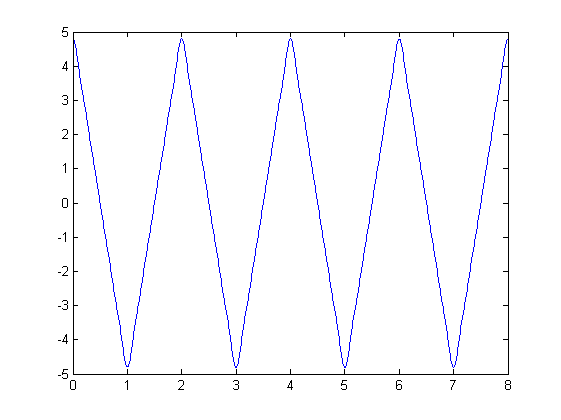
\includegraphics[scale=0.75]{img/q1-fourier-10.png}
	\caption{Décomposition en série de Fourier pour $k=1\cdots10$.}
	\label{fig:q1-fourier-10}
\end{figure}

Passons maintenant au cas général, c'est à
dire avec une origine des temps quelconque.
La série doit maintenant s'écrire sous la
forme
\begin{equation}
	u(t) = \sum_{k=-\infty}^\infty C_k e^{jk\omega t}.
	\label{eq:fourier-complex}
\end{equation}
Il s'agit ensuite d'exprimer $C_k$ en fonction
de $A_k$ et $B_k$ et de trouver une expression
simple pour $C_k$ faisant usage d'exponentielles
complexes. Pour ce faire, on utilise les relations
suivantes
\[ \cos(k\omega t) = \frac{e^{jk\omega t}+e^{-jk\omega t}}{2},\]
\[ \sin(k\omega t) = \frac{e^{jk\omega t}-e^{-jk\omega t}}{2j}\]
dans l'équation \ref{eq:fourier-real}
\[ u(t) = A_0 + \sum_{k=1}^{\infty} A_k\left(\frac{e^{jk\omega t}+e^{-jk\omega t}}{2}\right)
	+ \sum_{k=1}^{\infty} B_k\left(\frac{e^{jk\omega t}-e^{-jk\omega t}}{2j}\right). \]
On met un peu d'ordre dans cette expresion et on l'égalise 
ensuite à l'équation \ref{eq:fourier-complex}
\[ A_0 + \sum_{k=1}^{\infty} \frac{(A_k-jB_k)}{2}e^{jk\omega t}
	+ \sum_{k=1}^{\infty} \frac{(A_k+jB_k)}{2}e^{-jk\omega t} = 
	\sum_{k=-\infty}^\infty C_k e^{jk\omega t}.\]
De cette égalité, on retire
\[ C_k =
	\left\{
		\begin{array}{cl}
			A_0 & \text{ pour } n = 0 \\
			\frac{(A_k-jB_k)}{2} & \text{ pour } n = 1,2,3,\dots \\
			\frac{(A_{-k}+jB_{-k})}{2} & \text{ pour } n = -1,-2,-3,\dots
		\end{array}
	\right.
\]
En sachant que $A_0$, $A_k$ et $B_k$ sont
donnés respectivement par les équations
\ref{eq:fourier-constant}, \ref{eq:fourier-coef-cos}
et \ref{eq:fourier-coef-sin}, on pour calculer
$C_k$ dans les trois cas. On montre facilement que
\[ C_k = \frac{1}{T} \int_0^T u(t)e^{-jk\omega t}\dif t\]
dans les trois cas. Cette façon de procéder est tirée de 
\cite{complex-fourier-series}.
Il ne nous reste plus maintenant qu'à prouver
que $C_{-k} = C_k^*$ dans le cas d'un signal réel,
c'est à dire $u(t) \in \R$. On trouve très facilement que
\begin{equation}
	C_{-k} = \frac{1}{T} \int_0^T u(t)e^{jk\omega t}\dif t.
	\label{eq:c-minus}
\end{equation}
Il reste à calculer $C^*_k$

\[\arraycolsep=1.4pt\def\arraystretch{2.2}
	\begin{array}{cl}
		C_k^* &= 1/T \left(\int_0^T u(t)e^{-jk\omega t} \dif t\right)^* \\ 
					&= 1/T \int_0^T \left(u(t)e^{-jk\omega t}\right)^* \dif t \\
					&= 1/T \int_0^T (u(t))^*(e^{-jk\omega t})^* \dif t \\
					&= 1/T \int_0^T u(t)e^{jk\omega t} \dif t.
	\end{array}
\]

Cette expression est effectivement égale à
l'équation \ref{eq:c-minus}.

\biblio{problem1}
\end{document}